\section{Технологическая часть}
	\subsection{Средства реализации программного обеспечения}
		\subsubsection{Язык программирования}
			При разработке программного продукта был использован язык программирования Python (версия 3.7.2) \cite{python}.
			
			Данный выбор был сделан по следующим причинам.
			\begin{enumerate}
				\item[1)] Опыт работы с рассматриваемым языком.
				\item[2)] Поддержка ООП.
				\item[3)] Большое количество литературы, связанной с ЯП Python.
				\item[4)] Широкая применимость.
			\end{enumerate}
		
			В качестве среды разработки были использованы PyCharm \cite{pycharm} и Visual Studio Code \cite{vcode}, поскольку они бесплатны для студентов, удобны в процессе разработки и ранее активно использовались.

		\subsubsection{СУБД}
		Одними из наиболее популярных СУБД, используемых в настоящее время, являются Oracle, MySQL, Microsotf SQL сервер и PostgreSQL. В таблице \ref{cmptable} приведено их сравнение.
		
		\begin{table}[pt!] 
			\begin{center}
				\caption{Сравнение СУБД}
				\label{cmptable}
				\begin{tabular}{| c | l | l |}
					\hline
					\textbf{СУБД} 	& \textbf{Преимущества} & \textbf{Недостатки} \\
					\hline
					Oracle 			&  & - Платное использование \\ 
									& - Широкий функционал & - Необходимость в дополнительных \\
									& - Ориентирован на работу с большими &  ресурсах \\
									& БД & \\
					\hline
					MySQL 			& - Есть бесплатная версия &	- Есть платные версии для \\
									&  & коммерческого использования \\ 
									& - Исчерпывающая документация & - Для бесплатной версии доступна \\
									& - Простой интерфейс & только платная поддержка \\
									& - Хорошо справляется с большими & - Отсутствует встроенная поддержка \\
									& объёмами данных & XML \\
					\hline
					Microsotf SQL  	& - Низкий порог вхождения &	- Высокая цена для юридических \\
					сервер 			& - Стабильность в работе & лиц \\ 
									& - Возможность регулировать и  & - Требуется много дополнительных \\
									& отслеживать уровень & ресурсов \\ 
									& производительности &  \\
					\hline
					PostgreSQL 		& - Бесплатная & - Низкая скорость выполнения \\ 
									& - Подробная документация & пакетных операций\\
									& - Поддержка json & - Поддерживается не всеми \\
									&& библиотеками \\
					\hline
				\end{tabular}
			\end{center}
		\end{table}
	\newpage
	
	Поскольку есть опыт работы с такой СУБД, как PostgreSQL \cite{postgresql}, то это средство было выбрано для реализации текущей задачи.
	
	Что касается ORM (Object-relational mapping), то был выбран peewee \cite{peewee}, поскольку также хорошо знаком, так как активно использовался ранее.
	
	\subsubsection{Web-фреймворк}
	Django \cite{django} был выбран в качестве Web-фреймворка по следующим причинам.
	\begin{itemize}
		\item Использует шаблон проектирования MVC, который был выбран ранее.
		\item Работает с большим количеством дополнительных функций, которые значительно упрощают работу с аутентификацией пользователя, картами сайта и т.д.
		\item Масштабируемость.
	\end{itemize}

	\subsection{UML-диаграммы}
		\subsubsection{Компонент доступа к данным}
		Доступ к данным реализован с помощью паттерна проектирования Repository. Соответствующая UML-диаграмма представлена на рисунке \ref{fig6:image}.
		
		\begin{figure}[ph!]
			\centering
			\begin{center}
				{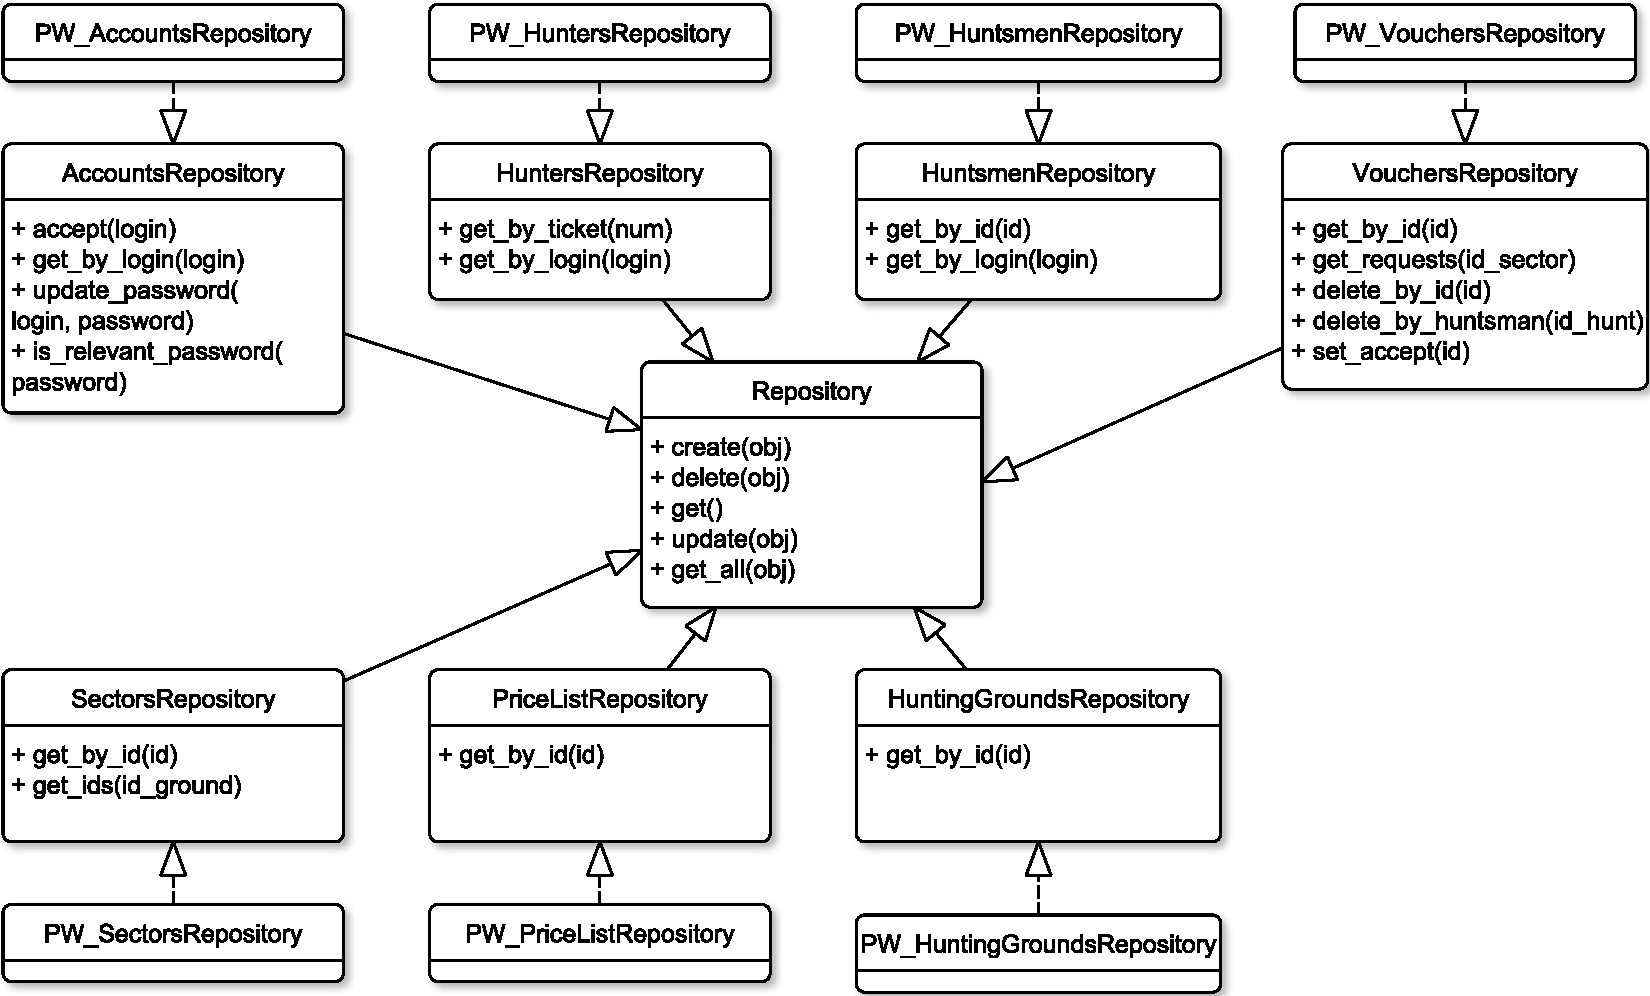
\includegraphics[scale=0.6]{schemes/uml_access_rep.pdf}}
				\caption{UML-диаграмма компонента доступа к данным}
				\label{fig6:image}
			\end{center}
		\end{figure}
		\newpage
	
		\subsubsection{Компонент бизнес-логики}
		Этот компонент выполняет основную обработку данных, соответствующая UML-диаграмма представлена на рисунке \ref{fig7:image}.
		
		\begin{figure}[ph!]
			\centering
			\begin{center}
				{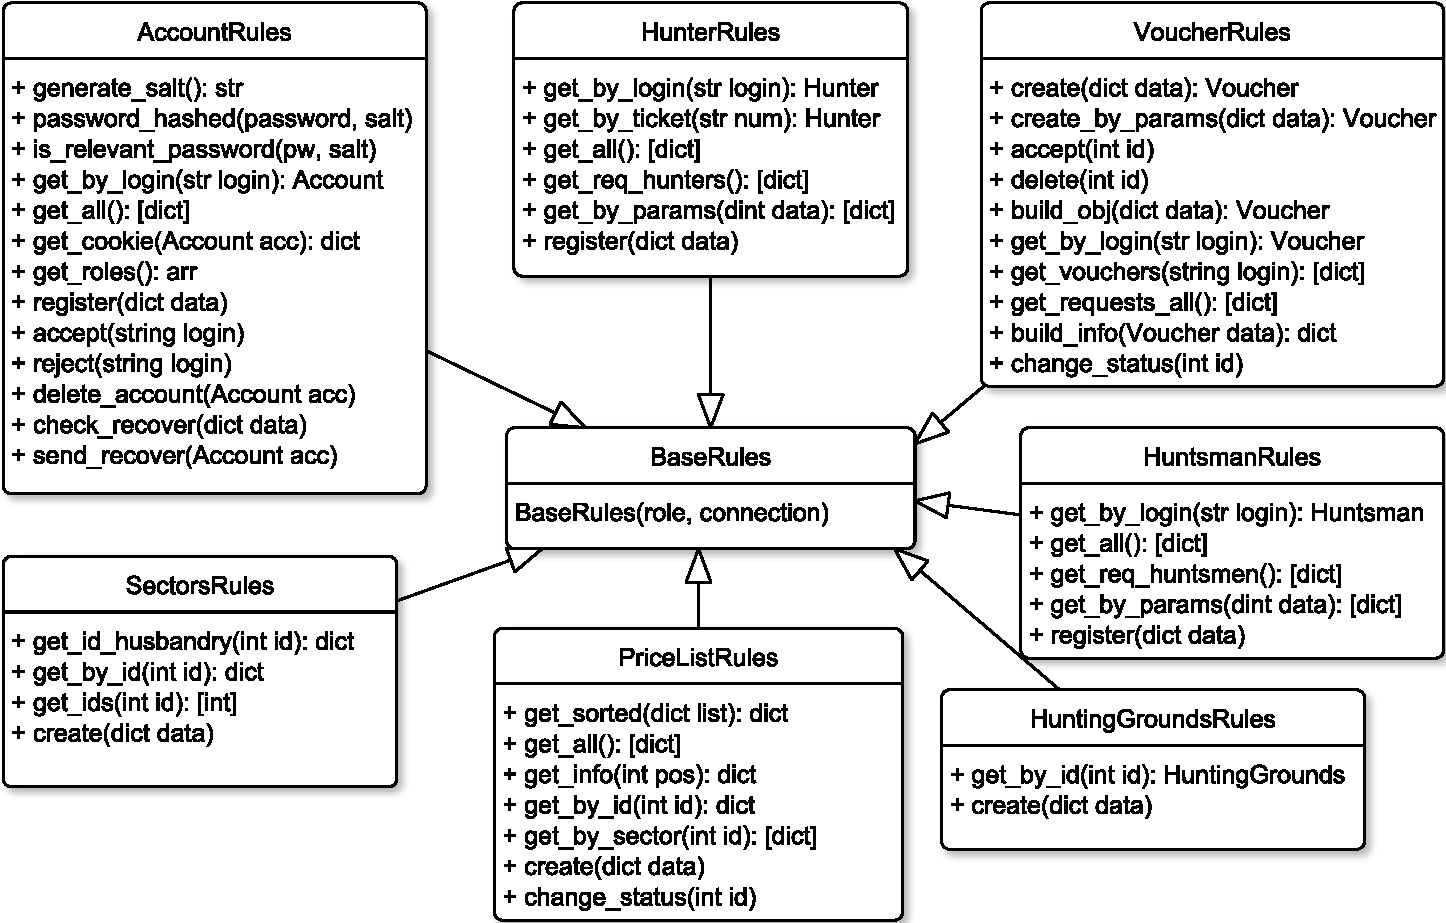
\includegraphics[scale=0.6]{schemes/uml_business.pdf}}
				\caption{UML-диаграмма компонента бизнес-логики}
				\label{fig7:image}
			\end{center}
		\end{figure}
	
		\subsubsection{Компонент представления}
		UML-диаграмма компонента, отвечающего за отображение web-страниц, изображена на рисунке \ref{fig8:image}.
		
		\begin{figure}[pt!]
			\centering
			\begin{center}
				{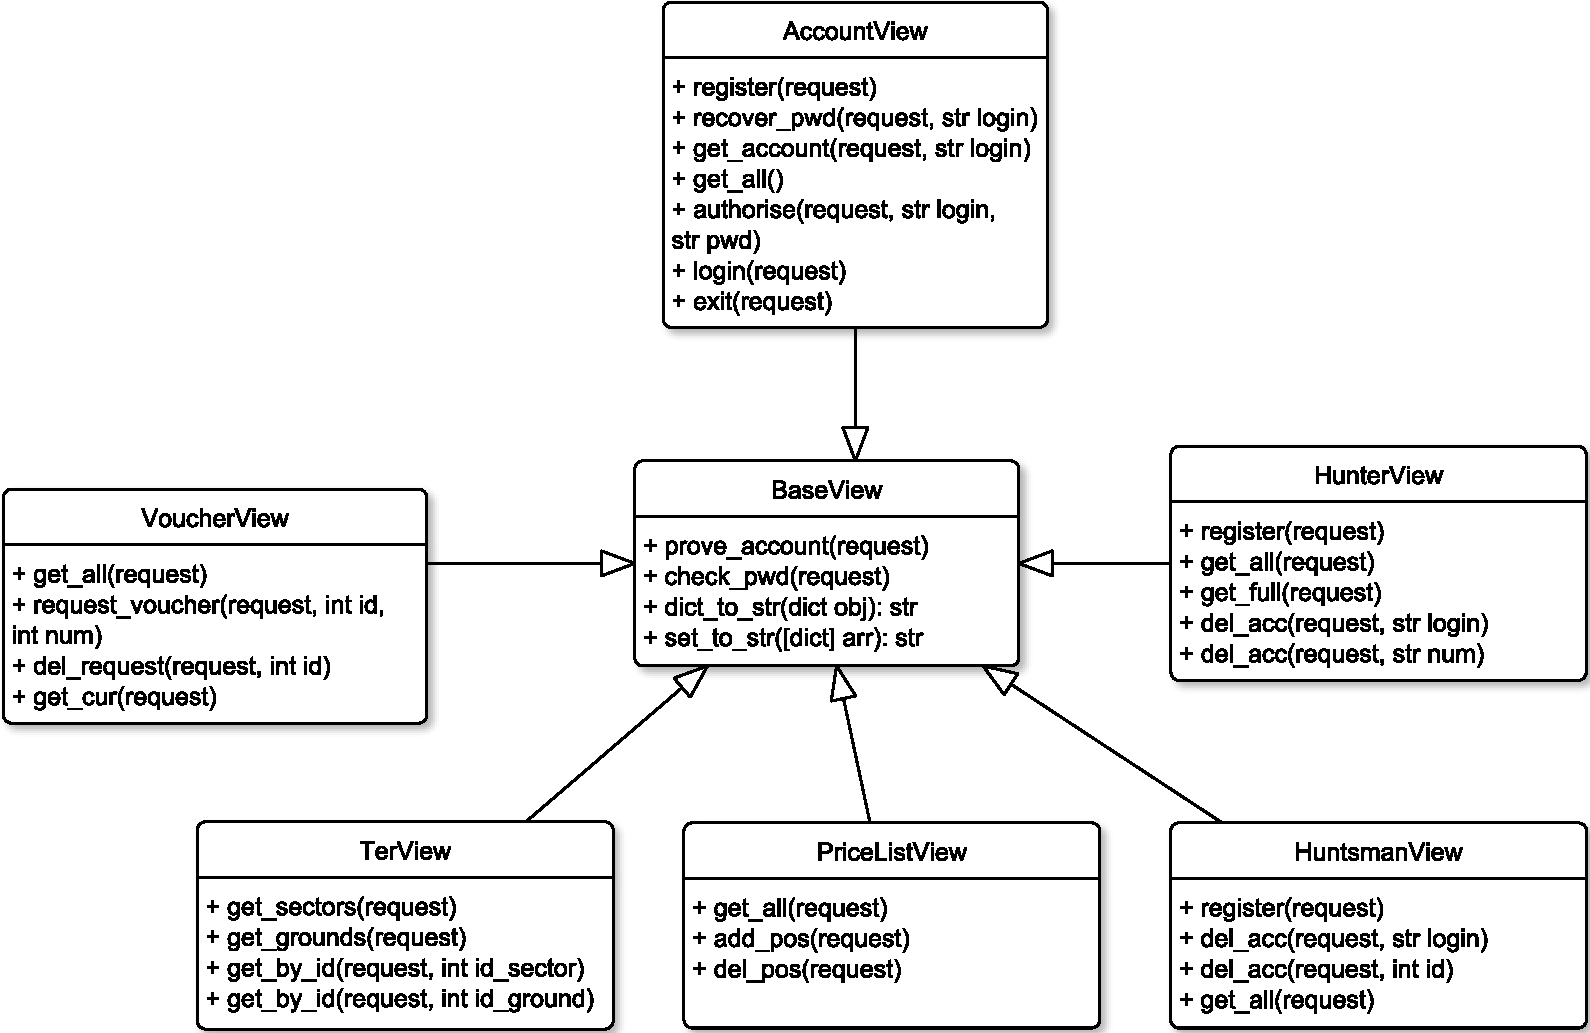
\includegraphics[scale=0.6]{schemes/webGUI.pdf}}
				\caption{UML-диаграмма компонента бизнес-логики}
				\label{fig8:image}
			\end{center}
		\end{figure}
		\newpage
	
		\subsubsection{Диаграмма приложения}
		Все приведённые выше UML-диаграммы \ref{fig6:image}-\ref{fig8:image} можно объединить в одну - диаграмму-приложения, которая находится на рисунке \ref{fig9:image}.
		
		\begin{figure}[ph!]
			\centering
			\begin{center}
				{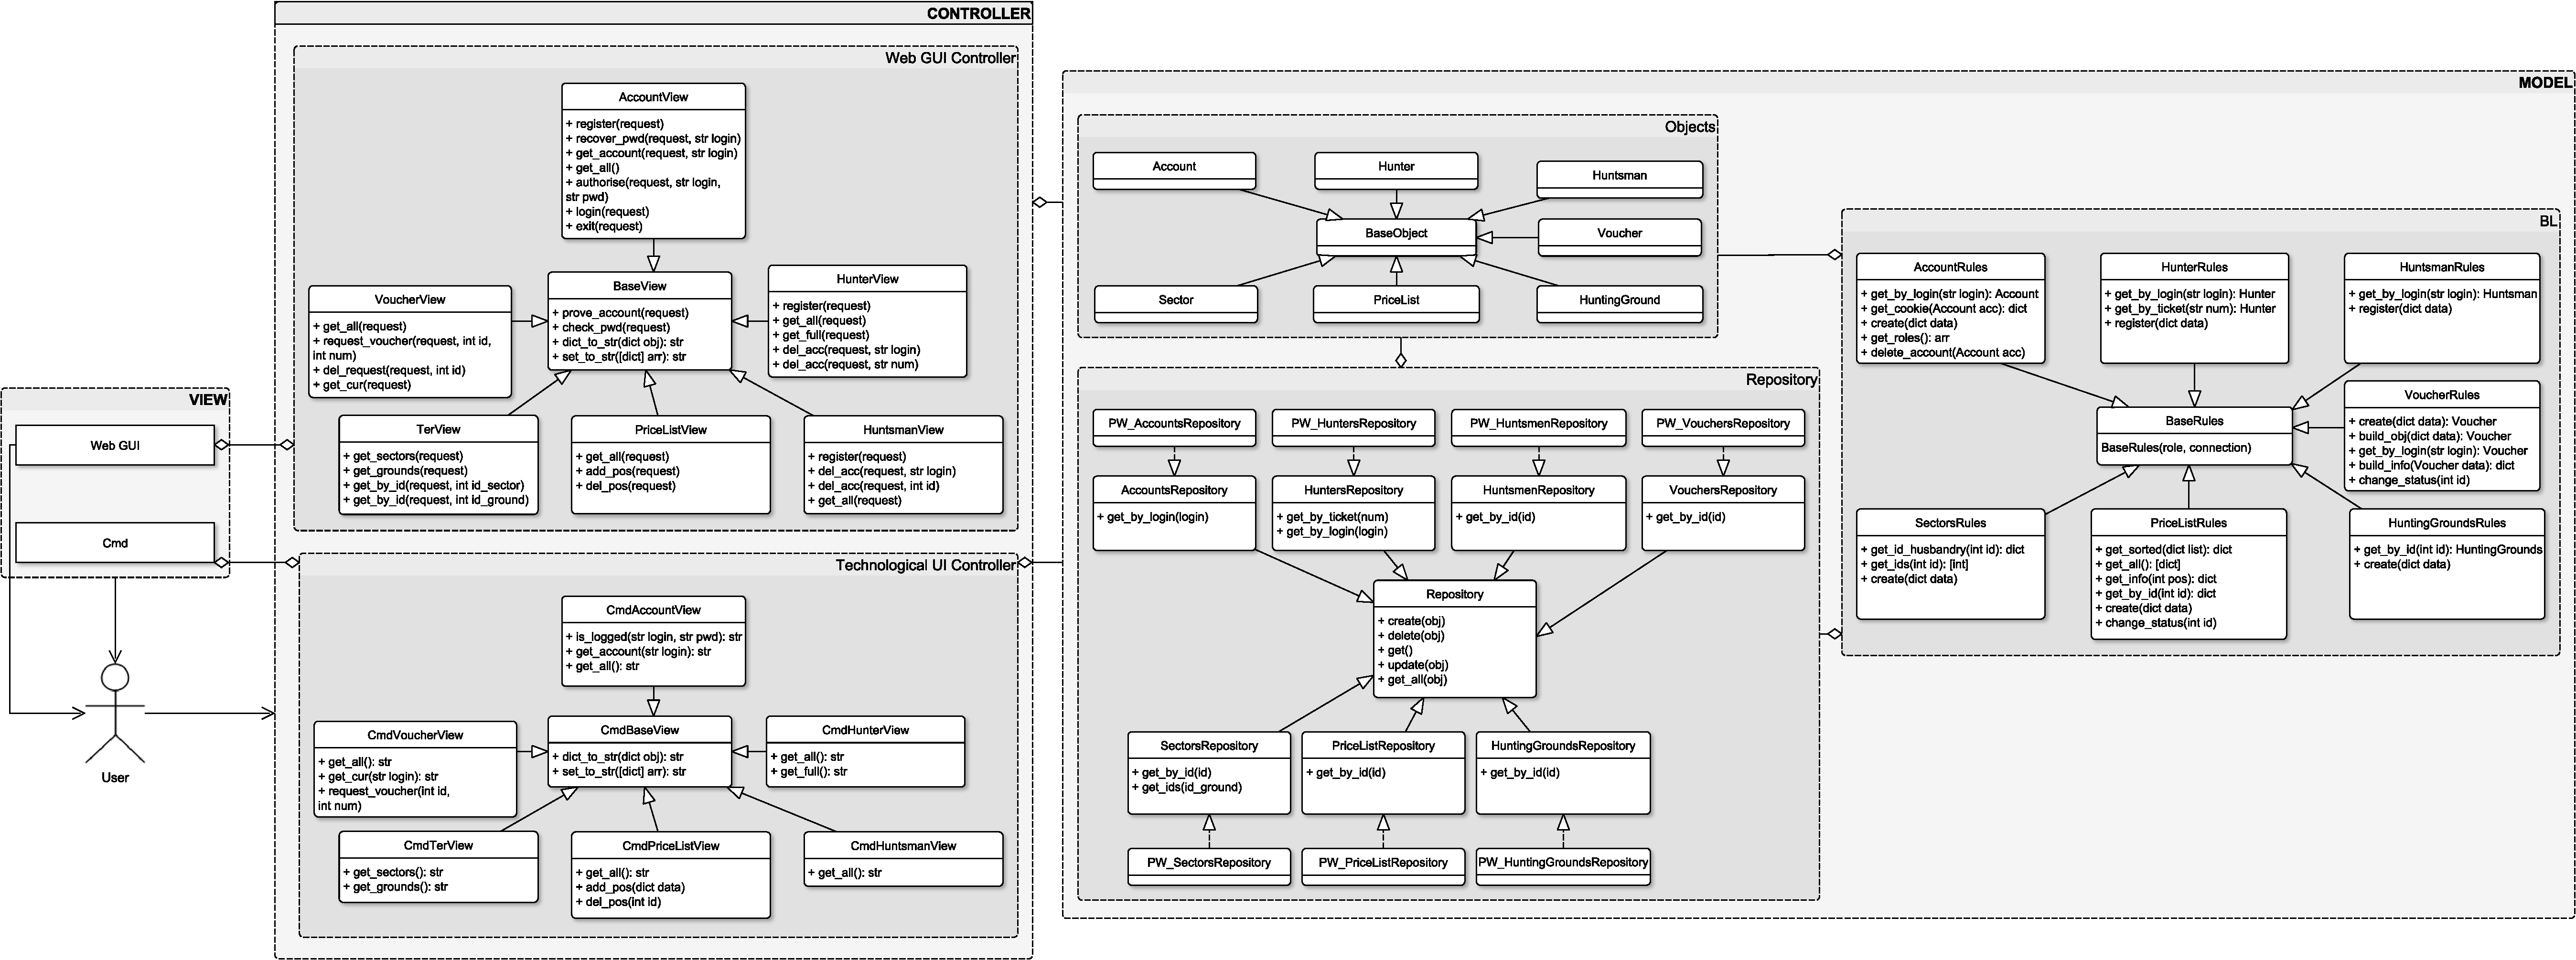
\includegraphics[scale=0.44, angle=90]{schemes/uml_full.pdf}}
				\caption{UML-диаграмма компонента бизнес-логики}
				\label{fig9:image}
			\end{center}
		\end{figure}
	\newpage
	
	\subsection{Реализация базы данных}
	!!!!!!!!!!!!!!!!!!!!!!!!!!!!!!!!!!!!!!!!!!!!!!!!!!!!!!!!!!!!!!!!!!!!!!!!!!!!!!!!!!!!!!!!!11
	\subsubsection{Создание таблиц}
	\subsubsection{Наполнение таблиц}
	\subsubsection{Реализация триггеров}
	\subsubsection{}
	
	\subsection{Интерфейс приложения}
	Для визуальной демонстрации приложения рассмотрим страницы, которые задействуются при оформлении путёвки. Сделать это может как охотник, так и егерь с администратором. 
	Для того, чтобы подать заявку на путёвку пользователь должен из верхнего меню (рисунок \ref{fig10:image}) навести мышкой на пункт <<ПУТЁВКИ>>, и затем, из выпадающего списка выбрать действие <<Купить>>.
	
	\begin{figure}[h]
		\centering
		\begin{center}
			{\includegraphics[scale=0.34]{schemes/screens/start.png}}
			\caption{Переход на страницу подачи заявки на путёвку}
			\label{fig10:image}
		\end{center}
	\end{figure}

	После этого охотник попадает на страницу, изображенную на рисунке \ref{fig11:image}. На ней приведён полный список всех доступных путёвок по всем хозяйствам и секторам. Используя мышь или правую полосу прокрутки можно ознакомиться со всем списком. 
	
	Каждая позиция из списка содержит информацию о месте (название хозяйства) и номере сектора, названии животного, на которого выдаётся разрешение, и цена за 1 единицу. 
	
	В поле <<Количество>> пользователь может указать, на сколько животных он хотел бы оформить путёвку. Для этого достаточно нажать кнопкой мыши на это поле в соответствующей строке из прайс-листа. Пользователь может указать число от 1 до 99, причём чтобы контролировать число отстреленных животных только егерь, закрепленный за данным сектором, или администратор может принимать решение одабривать такую заявку или, наоборот, отклонить. 
	
	\begin{figure}[h]
		\centering
		\begin{center}
			{\includegraphics[scale=0.34]{schemes/screens/menu.png}}
			\caption{Прайс-лист доступных путёвок}
			\label{fig11:image}
		\end{center}
	\end{figure}

	Если охотник введёт некорректные данные (например, как на рисунке \ref{fig12:image}) и попробует оформить путёвку, нажав на <<Отправить заявку>>, то он увидит сообщение о невалидности данных (рисунок \ref{fig13:image}).
	
	\begin{figure}[h]
		\centering
		\begin{center}
			{\includegraphics[scale=0.34]{schemes/screens/wrong_num.png}}
			\caption{Некорректный ввод данный в поле <<Количество>>}
			\label{fig12:image}
		\end{center}
	\end{figure}

	\begin{figure}[h]
		\centering
		\begin{center}
			{\includegraphics[scale=0.34]{schemes/screens/msg_error.png}}
			\caption{Сообщение о некорректном вводе данных}
			\label{fig13:image}
		\end{center}
	\end{figure}
	\newpage
	
	Также пользователь может воспользоваться поиском по названию субъекта (рисунок \ref{fig14:image}).
	
	\begin{figure}[h]
		\centering
		\begin{center}
			{\includegraphics[scale=0.3245]{schemes/screens/find.png}}
			\caption{Демонстрация работы поиска}
			\label{fig14:image}
		\end{center}
	\end{figure}
	\newpage

	Если же охотник ввёл корректное число животных (рисунок \ref{fig15:image}) и нажал на <<Отправить заявку>>, то в этом случае на странице появляется соответствующее сообщение, как на рисунке \ref{fig16:image}.
	
	\begin{figure}[h]
		\centering
		\begin{center}
			{\includegraphics[scale=0.34]{schemes/screens/right_data.png}}
			\caption{Корректно оформленная заявка}
			\label{fig15:image}
		\end{center}
	\end{figure}

	\begin{figure}[h]
		\centering
		\begin{center}
			{\includegraphics[scale=0.34]{schemes/screens/msg_right.png}}
			\caption{Сообщение об успешном оформлении заявки}
			\label{fig16:image}
		\end{center}
	\end{figure}

	Просмотреть все свои заявки, а также уже одобренные путёвки охотник может, кликнув на поле <<Просмотреть свои>> (рисунок \ref{fig17:image}).
	
	\begin{figure}[h]
		\centering
		\begin{center}
			{\includegraphics[scale=0.34]{schemes/screens/to_have.png}}
			\caption{Переход на страницу всех заявок и одобренных путёвок}
			\label{fig17:image}
		\end{center}
	\end{figure}

	В результате охотник попадает на страницу, изображённую на рисунке \ref{label}. На ней сначала указаны все одобренные текущему охотнику путёвки (то есть, по ним он уже может охотиться), и ниже все заявки. Также по каждой из этих двух таблиц можно осуществить поиск по субъекту. На рисунке \ref{fig15:image} указано, какая именно позиция из прайс-листа была выбрана, и уже на этой странице можно увидеть эту заявку (выделена белым цветом).
	
	\begin{figure}[h]
		\centering
		\begin{center}
			{\includegraphics[scale=0.34]{schemes/screens/all_vouchers.png}}
			\caption{Всех заявки и одобренные путёвок текущего охотника}
			\label{fig18:image}
		\end{center}
	\end{figure}

	Если по какой-то причине пользователь передумал оформлять путёвку, то он может отозвать оформленную ранее заявку, нажав на кнопку в столбце <<Отозвать>>. 
	
	Для наглядности была отозвана путёвка на гуся. После этого страница выглядит так, как показано на рисунке \ref{fig19:image}. 
	
	Показателем того, что операция прошла успешно, является соответствующее сообщение и отсутствие выбранной позиции на странице. 
	
	Удалить или отозвать уже одобренные путёвки охотник не может, так как считается, что покупка уже совершена, а закрыть её по определённым причинам может только егерь, закреплённый за сектором, куда была выдана путёвка, или администратор.
	
	\begin{figure}[h]
		\centering
		\begin{center}
			{\includegraphics[scale=0.34]{schemes/screens/after_del_huntsman.png}}
			\caption{Страница после того, как была отозвана заявка}
			\label{fig19:image}
		\end{center}
	\end{figure}


	
	
		
		 
		
	